% Drawing 142/02-2 -- folder 142, batch 02, archive page 25 (PDF page 26).
% Transcription: même sphère que p.~23, à laquelle s'ajoutent sur l'équateur trois nouveaux sommets $Q_0$, $Q_1$, $Q_\infty$ et des arcs $c_i^{\pm}$ qui les relient aux sommets $R^{\pm}$ voisins. Légende : $\mathrm{II}_J$.
% Kind: sphere with marked points, small circles and arrows. Method 2 (schematic redraw from the facsimile). Status: ok.
% Notes: As 02-1 with the signs +/- for omega, omega'; the new vertices Q_0, Q_1, Q_infty on the equator and the arrows c_i^+- joining them to the R. The legend II_J (below-left of the sphere) is text, not drawn. Q_1 sits at the left end of the equator, its label being c_1^+ there.
% Coordinates: 1 unit = 1 mm = 1/100 of the crop width (bbox in page fractions: [0.1, 0.08, 0.34, 0.2]).
% Redrawn by Claude (claude-opus-5-5), issue #73, 2026-11-07; not checked by a human; not compiled (no TeX in the session).
% Rights: reproduces part of the work -- behind RENDER_TRANSCRIPTS, never published by itself.
\documentclass[tikz,border=3pt]{standalone}
\usepackage{amsmath,amssymb}
\usetikzlibrary{patterns,arrows.meta}
\tikzset{pencil/.style={black!45}, struck/.style={black!35}, mark/.style={circle,draw,inner sep=1.3pt}, pt/.style={circle,fill,inner sep=0.9pt}, opt/.style={circle,draw,fill=white,inner sep=1.1pt}}
\begin{document}
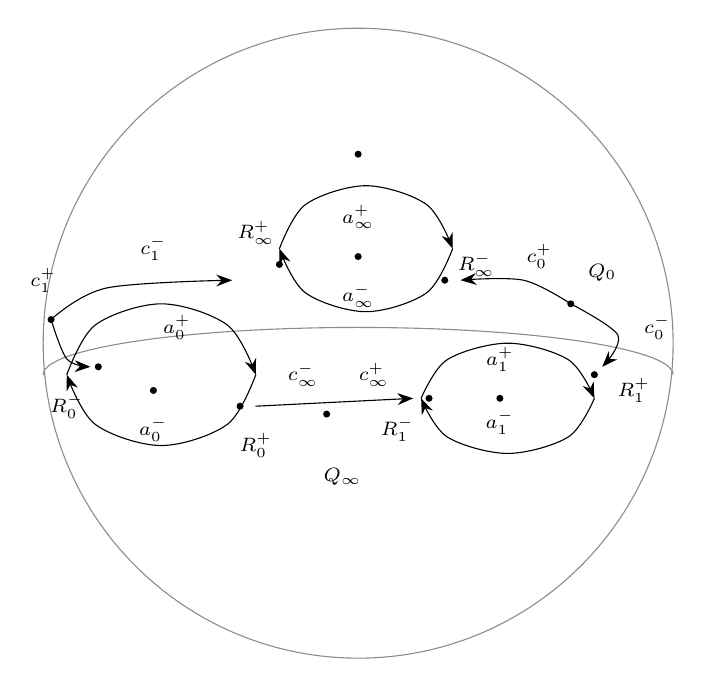
\begin{tikzpicture}[x=1mm,y=1mm,line cap=round,line join=round,font=\scriptsize]
\draw[pencil] (57,-48) circle[radius=40];
\draw[pencil] (97,-52) arc[start angle=0, end angle=180, x radius=40, y radius=6];
\node[pt] at (57,-24) {};
\node[pt] at (57,-37) {};
\node[pt] at (31,-54) {};
\node[pt] at (75,-55) {};
\draw[-{Stealth[length=2mm]}] plot[smooth, tension=0.55] coordinates {(47,-36) (50.3,-30.4) (58,-28) (65.7,-30.4) (69,-36)};
\draw[-{Stealth[length=2mm]}] plot[smooth, tension=0.55] coordinates {(69,-36) (65.7,-41.6) (58,-44) (50.3,-41.6) (47,-36)};
\draw[-{Stealth[length=2mm]}] plot[smooth, tension=0.55] coordinates {(20,-52) (23.6,-45.7) (32,-43) (40.4,-45.7) (44,-52)};
\draw[-{Stealth[length=2mm]}] plot[smooth, tension=0.55] coordinates {(44,-52) (40.4,-58.3) (32,-61) (23.6,-58.3) (20,-52)};
\draw[-{Stealth[length=2mm]}] plot[smooth, tension=0.55] coordinates {(65,-55) (68.3,-50.1) (76,-48) (83.7,-50.1) (87,-55)};
\draw[-{Stealth[length=2mm]}] plot[smooth, tension=0.55] coordinates {(87,-55) (83.7,-59.9) (76,-62) (68.3,-59.9) (65,-55)};
\node[pt] at (47,-38) {};
\node[pt] at (68,-40) {};
\node[pt] at (24,-51) {};
\node[pt] at (42,-56) {};
\node[pt] at (66,-55) {};
\node[pt] at (87,-52) {};
\node[pt] at (53,-57) {};
\node[pt] at (84,-43) {};
\node[pt] at (18,-45) {};
\draw[-{Stealth[length=2mm]}] plot[smooth, tension=0.55] coordinates {(18,-45) (25,-41) (41,-40)};
\draw[-{Stealth[length=2mm]}] (44,-56) -- (64,-55);
\draw[-{Stealth[length=2mm]}] plot[smooth, tension=0.55] coordinates {(84,-43) (78,-40) (70,-40)};
\draw[-{Stealth[length=2mm]}] plot[smooth, tension=0.55] coordinates {(84,-43) (90,-47) (88,-51)};
\draw[-{Stealth[length=2mm]}] plot[smooth, tension=0.55] coordinates {(18,-45) (20,-50) (23,-51)};
\node[inner sep=1pt] at (44,-34) {\scriptsize $R_\infty^{+}$};
\node[inner sep=1pt] at (72,-38) {\scriptsize $R_\infty^{-}$};
\node[inner sep=1pt] at (20,-56) {\scriptsize $R_0^{-}$};
\node[inner sep=1pt] at (44,-61) {\scriptsize $R_0^{+}$};
\node[inner sep=1pt] at (62,-59) {\scriptsize $R_1^{-}$};
\node[inner sep=1pt] at (92,-54) {\scriptsize $R_1^{+}$};
\node[inner sep=1pt] at (57,-32) {\scriptsize $a_\infty^{+}$};
\node[inner sep=1pt] at (57,-42) {\scriptsize $a_\infty^{-}$};
\node[inner sep=1pt] at (34,-46) {\scriptsize $a_0^{+}$};
\node[inner sep=1pt] at (31,-59) {\scriptsize $a_0^{-}$};
\node[inner sep=1pt] at (75,-50) {\scriptsize $a_1^{+}$};
\node[inner sep=1pt] at (75,-58) {\scriptsize $a_1^{-}$};
\node[inner sep=1pt] at (17,-40) {\scriptsize $c_1^{+}$};
\node[inner sep=1pt] at (31,-36) {\scriptsize $c_1^{-}$};
\node[inner sep=1pt] at (50,-52) {\scriptsize $c_\infty^{-}$};
\node[inner sep=1pt] at (59,-52) {\scriptsize $c_\infty^{+}$};
\node[inner sep=1pt] at (55,-65) {\scriptsize $Q_\infty$};
\node[inner sep=1pt] at (80,-37) {\scriptsize $c_0^{+}$};
\node[inner sep=1pt] at (88,-39) {\scriptsize $Q_0$};
\node[inner sep=1pt] at (95,-46) {\scriptsize $c_0^{-}$};
\end{tikzpicture}
\end{document}
